\section[Electromagnetic calorimeters (Elton/Colin)] {Electromagnetic calorimeters \label{sec:calorimeters}}
\subsection[Barrel calorimeter ]{Barrel calorimeter \label{sec:bcal}}
The barrel calorimeter (BCAL) detects photon showers with energies between 0.05 GeV and several GeV, $11^{\circ}$--$126^{\circ}$ in polar angle, and $0^{\circ}$--$360^{\circ}$ in azimuthal angle. Details of the design, construction and performance of the BCAL can be found in Ref.\cite{BEATTIE201824}. The containment of showers depends on the angle of particle incidence, with a thickness of $15.3$ radiation lengths for particles entering normal to the calorimeter face and reaching up to 67 radiation lengths at $14^{\circ}$. Geometrically, the BCAL consists of 48 optically isolated modules each with a trapezoidal cross section, forming a  390~cm-long cylindrical shell having inner and outer radii of 65~cm and 90~cm, respectively. The fibers run parallel to the cylindrical axis of the detector.  Details of the end of the calorimeter with light guides, light sensors and electronics are shown in  Fig.\,\ref{fig:bcal:bcal_assemblies}.

\begin{figure}[http]\centering
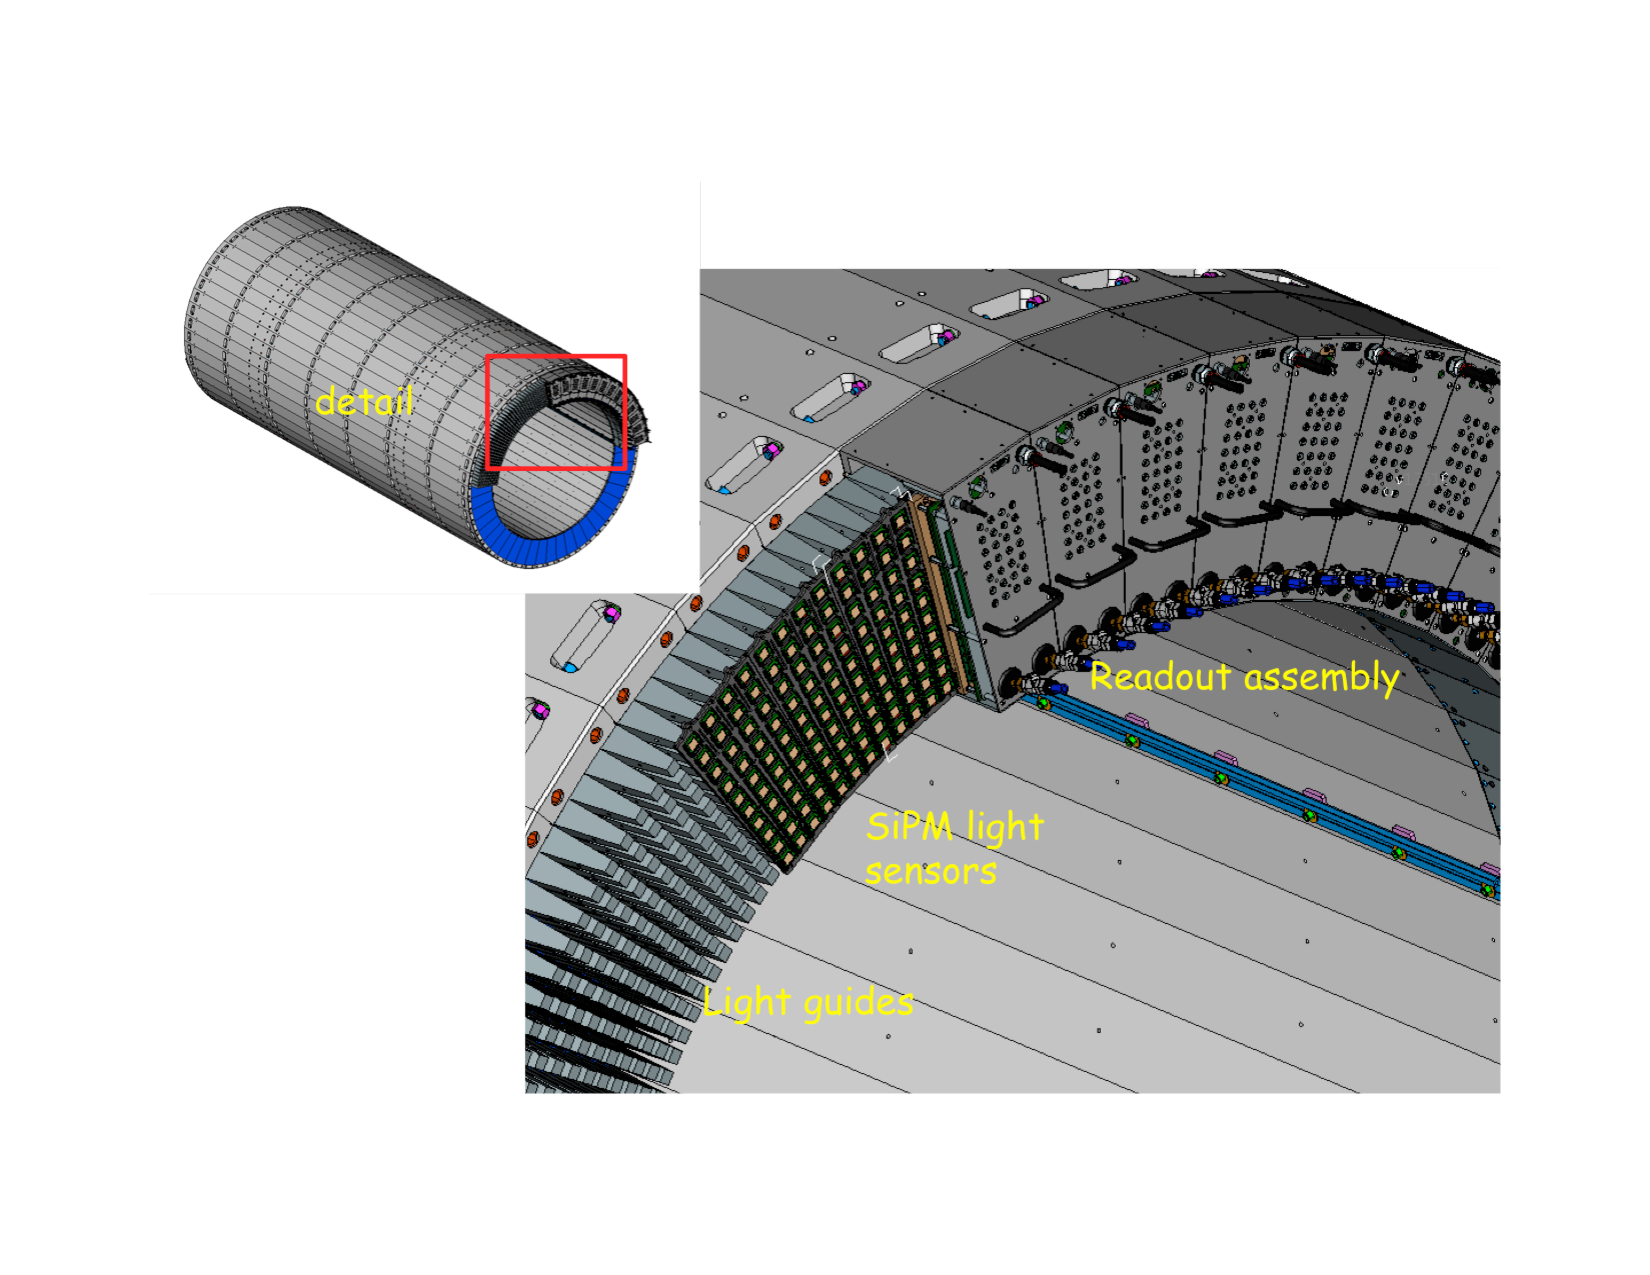
\includegraphics[scale=0.4]{figures/bcal_assemblies.pdf}
\caption{\label{fig:bcal:bcal_assemblies}
   Three-dimensional rendition of the light guides mounted at the end of the 
   BCAL, as well as the readout assemblies mounted over them. The 
   readout assemblies contain the 
   SiPMs and their electronics.  (Color online)
  }
\end{figure}
The BCAL is constructed as a lead and  scintillating-fiber matrix
and read out with silicon photomultiplier (SiPM) arrays. The matrix consists of 0.5 mm-thick grooved lead sheets and 1.0 mm-diameter Kuraray SCSF-78MJ multi-clad fibers.
Each module has approximately 185 layers and 15,000 fibers.
Particles impinge on the detector over a wide range of angles, from normal incidence at 90 degrees down to 11.5 degrees, which defines a geometry that is fairly unique among calorimeters. 

The light is collected via small light guides at each end of the module and transported to the SiPMs, which were chosen due to their insensitivity to magnetic fields. 
The light sensors are Hamamatsu S12045(X) Multi-Pixel Photon Counter (MPPC) arrays \footnote{Hamamatsu Corporation, Bridgewater, NJ 08807, USA \\ (\url{http://sales.hamamatsu.com/en/home.php)}.}, 
which are $4\times4$ arrays of $3\times3$ mm$^2$ tiles \cite{hdnote2913}.
The SiPMs were tested extensively before acceptance
\cite{Barbosa2012100,Qiang2013234,soto,Soto201489,doi:10.1063/1.4955340}.
Four thousand units were purchased and 3840 are installed in the detector.
The gain of the SiPM depends on the voltage above the breakdown voltage, which is about 70~V. We operate them at 1.4 V over the breakdown voltage, which was selected to reduce the effect of readout thresholds. Even at this relatively high over-bias, the noise level is dominated by fluctuations in the electronics baseline and not by single-pixel noise. In order to keep a constant gain, 
we maintained the temperature within practical limits ($\pm$ 2$^\circ$C) 
using a chilled water system and then stabilized the gain 
using a custom circuit that adjusted the bias voltage based on the measured temperature. Two stages of preamplifiers and summing electronics are attached to the sensors. In order to reduce the number of signals that are digitized, circuits sum the outputs of the preamplifiers in groups of radial columns, with coarser granularity away from the target. The layer closest to the target consists of a single SiPM. On the end of each module, forty SiPMs generate sixteen signals that are delivered to flash ADCs (FADCs) and twelve signals that are discriminated and then recorded with pipeline TDCs. The FADCs and TDCs are conveniently located on the floor of the experimental hall in VXS crates.
  
\subsection{Forward calorimeter \label{sec:fcal}}
The forward calorimeter (FCAL) detects photon showers with energies ranging from 0.1 GeV to several GeV between $1^{\circ}$--$11^{\circ}$. The FCAL is located 5.6 m downstream from the center of the GlueX target and consists of 2800 lead glass blocks stacked in a circular array that has a diameter of 2.4 m, as seen in Fig. \ref{}. Optically coupled to each block is a FEU 84-3 photomultiplier tube (PMT). 

The lead glass and PMTs are the same components that were used in the RADPHI and E852 experiments \cite{JONES2007384}, \cite{CRITTENDEN1997377}. Each PMT is powered by a Crockcroft--Walton (CW) base, with each consuming 0.2 W of power each \cite{BRUNNER1998466}. The use of CW bases eliminates the need for a 2400 channel high voltage power system. 

\subsection{Electronics \label{sec:calelectronics}}
Custom readout electronics are mounted in standard VXS crates and include 
JLab 12-bit 250~MHz FADCs \cite{hdnote1022}, discriminators \cite{hdnote2511} and F1 Time-to-Digital Converters (TDCs) \cite{hdnote1021}. The maximum input scale of the FADCs (4095 counts) is set to 2\,V.
The FADCs sample each calorimeter channel every 4\,ns and generate raw waveforms consisting of 100 samples 
 (400\,ns), which are available for further processing by the firmware upon a trigger signal if there is a threshold crossing. The firmware computes several derived features of the pulse: pedestal, peak value, integral over a selected window, and
 time of the half-way point on the leading edge. At most one pulse is extracted from each readout window. These  pulse features constitute the raw data that is read out from the FADC. 
 Optionally, the full waveforms can be read out for diagnostic purposes
 and to check the firmware output against the offline emulation of the parameter extraction. We record full waveforms in less than about 1\% of the production runs. The pedestals are determined for each channel event-by-event, appropriately scaled, and then subtracted from the peak and integral to obtain signals proportional to the energy deposited in the calorimeter. 
 Pulses are identified by the first sample that exceeds a threshold, 
 currently set to 105 (110??) counts for the BCAL (FCAL). Typical pedestal widths are $\sigma\sim$1.2-1.3 (1.2??) counts for the BCAL (FCAL). The integral is determined using a fixed number of samples relative to the threshold crossing, 
 which was determined by maximizing the ratio of signal to pedestal noise. 
 The integration window begins one (3??) samples before the threshold time and extends to 26 (40??) samples after the threshold time for the BCAL (FCAL). 
 %See Fig.\,\ref{fig:Plot_waveform10}.
 The algorithm that determines the time of the pulse is pulse-height independent and therefore no time-walk correction is required for the FADC times.

The outputs of the three inner layers of the BCAL cells are also connected leading-edge discriminators, which feed the JLab F1 TDCs. 
 The discriminator thresholds are typically set to about 35 mV, but are adjusted
 channel by channel.  The pulse times are recorded relative to the trigger in a 12-bit word. Multiple hits, up to eight, may be recorded per channel per event, but are culled at a later time by comparison to FADC times. The nominal least count is configured to 58\,ps.


\subsection[Calibrati0n and monitoring]{Calibration and monitoring \label{sec:calcalib}}
The relative gains of the calorimeters are monitored using a modular LED-driver system \cite{Anassontzis201441}. The control system is the same for both calorimeters, but the arrangement of LEDs is tailored to the geometry of each detector. In the BCAL, there is one LED inserted into each light guide, which can be used to monitor each individual SiPM and its partner at the far end of the module.
Due to geometry the illumination varies considerably from channel to channel. 
The average stability of the detector over a period of ten days is better than 1\% and the fractional root-mean-square (RMS) deviations of the mean for each SiPM during a single data from the average over the run period is typically less than 2\%.

For the FCAL, we installed four plexiglass panes, each covering the upstream end of one quadrant of the FCAL. Each pane is illuminated by forty LEDs, ten violet, ten blue and twenty green. The different colors are used to monitor the light transmission of the lead glass blocks. 


\subsection{Performance \label{sec:calperformance}}
The performance of the calorimeter is summarized by its ability to measure the energy, position and timing of electromagnetic showers. 
The energy resolution of the BCAL was extracted from the measured $\pi^0$ and
$\eta$ mass distributions, which yielded consistent results. To study the $\eta$ mass resolution, we selected events
using kinematic fits to $\gamma p \rightarrow p \pi^+ \pi^- \gamma \gamma$. 
This reaction provides a fairly clean sample of $\eta$'s where both photons are recorded in the BCAL. The charged tracks were used to determine the event vertex needed to reconstruct the two-photon invariant mass.  The MC simulation 
generated $\gamma p \rightarrow p \pi^+ \pi^- \eta$ events, with $\eta\rightarrow \gamma\gamma$, where the kinematics were chosen to approximate the experimental distributions. The fitted Gaussian widths are shown in Fig.\,\ref{fig:bcal:eta_resolution}a as a function of the photon energy, both for data and simulation. 
The single-photon energy resolution can be determined from the $\eta$ width by neglecting contributions from the opening angle.
This is shown in Fig.\,\ref{fig:bcal:eta_resolution}b, where one can see that the resolution extracted from the data is only slightly above the MC. If we average the response over the $\pi^0$ and $\eta$ spectra we find 
$\sigma_E/E$=5.2\%/$\sqrt{E(\rm{GeV})} \oplus$ 3.6\%. The large constant term is artificially large because of the averaging over angles; at a single angle in the forward direction, the constant term is less than 1.7\%.

The position resolution ($\sim$\,2.5 cm) is determined by the timing resolution of the system, which was determined to be $\sigma$\,=\,150\,ps at 1\,GeV.
 


\begin{figure}[tbh]\centering
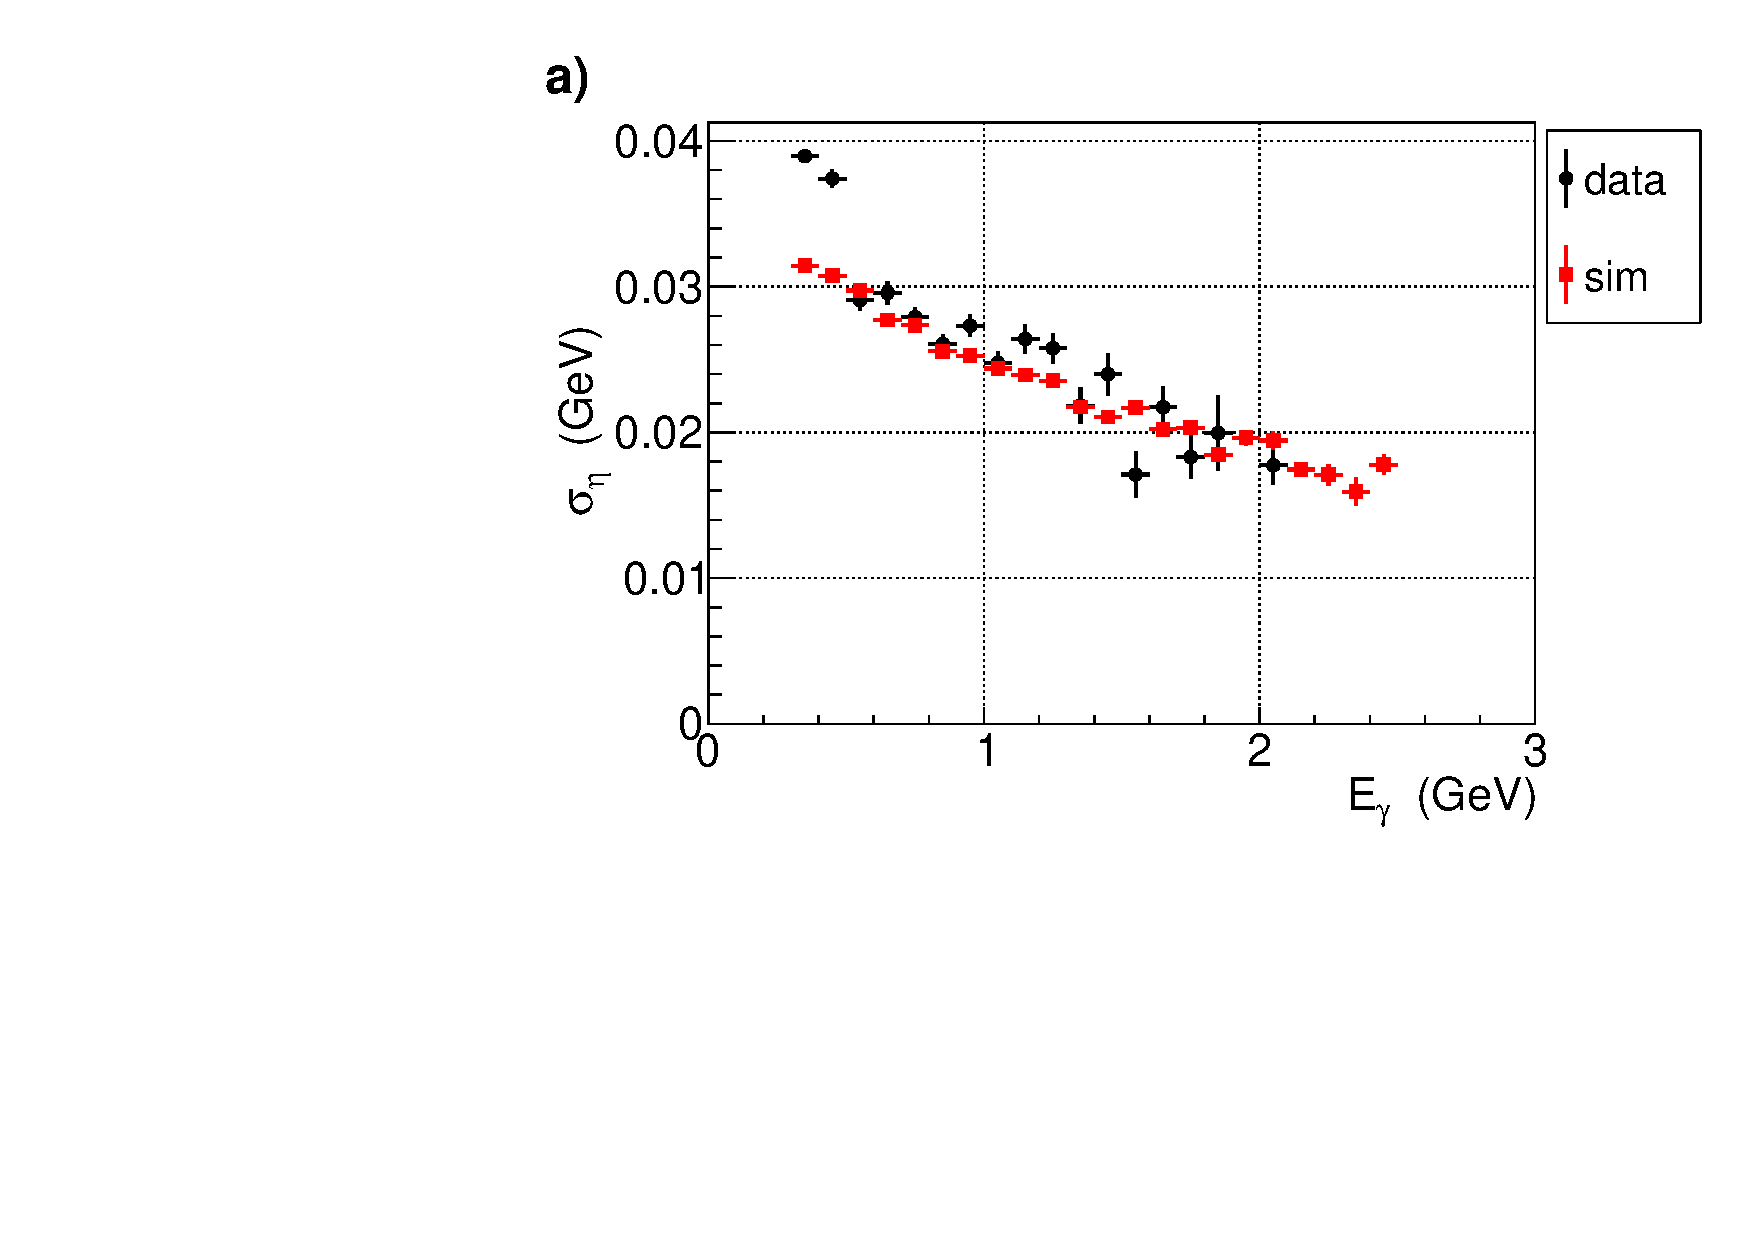
\includegraphics[width=0.45\textwidth]{figures/mcsmear50_37_gPsym100_etamass_sigma.pdf}   
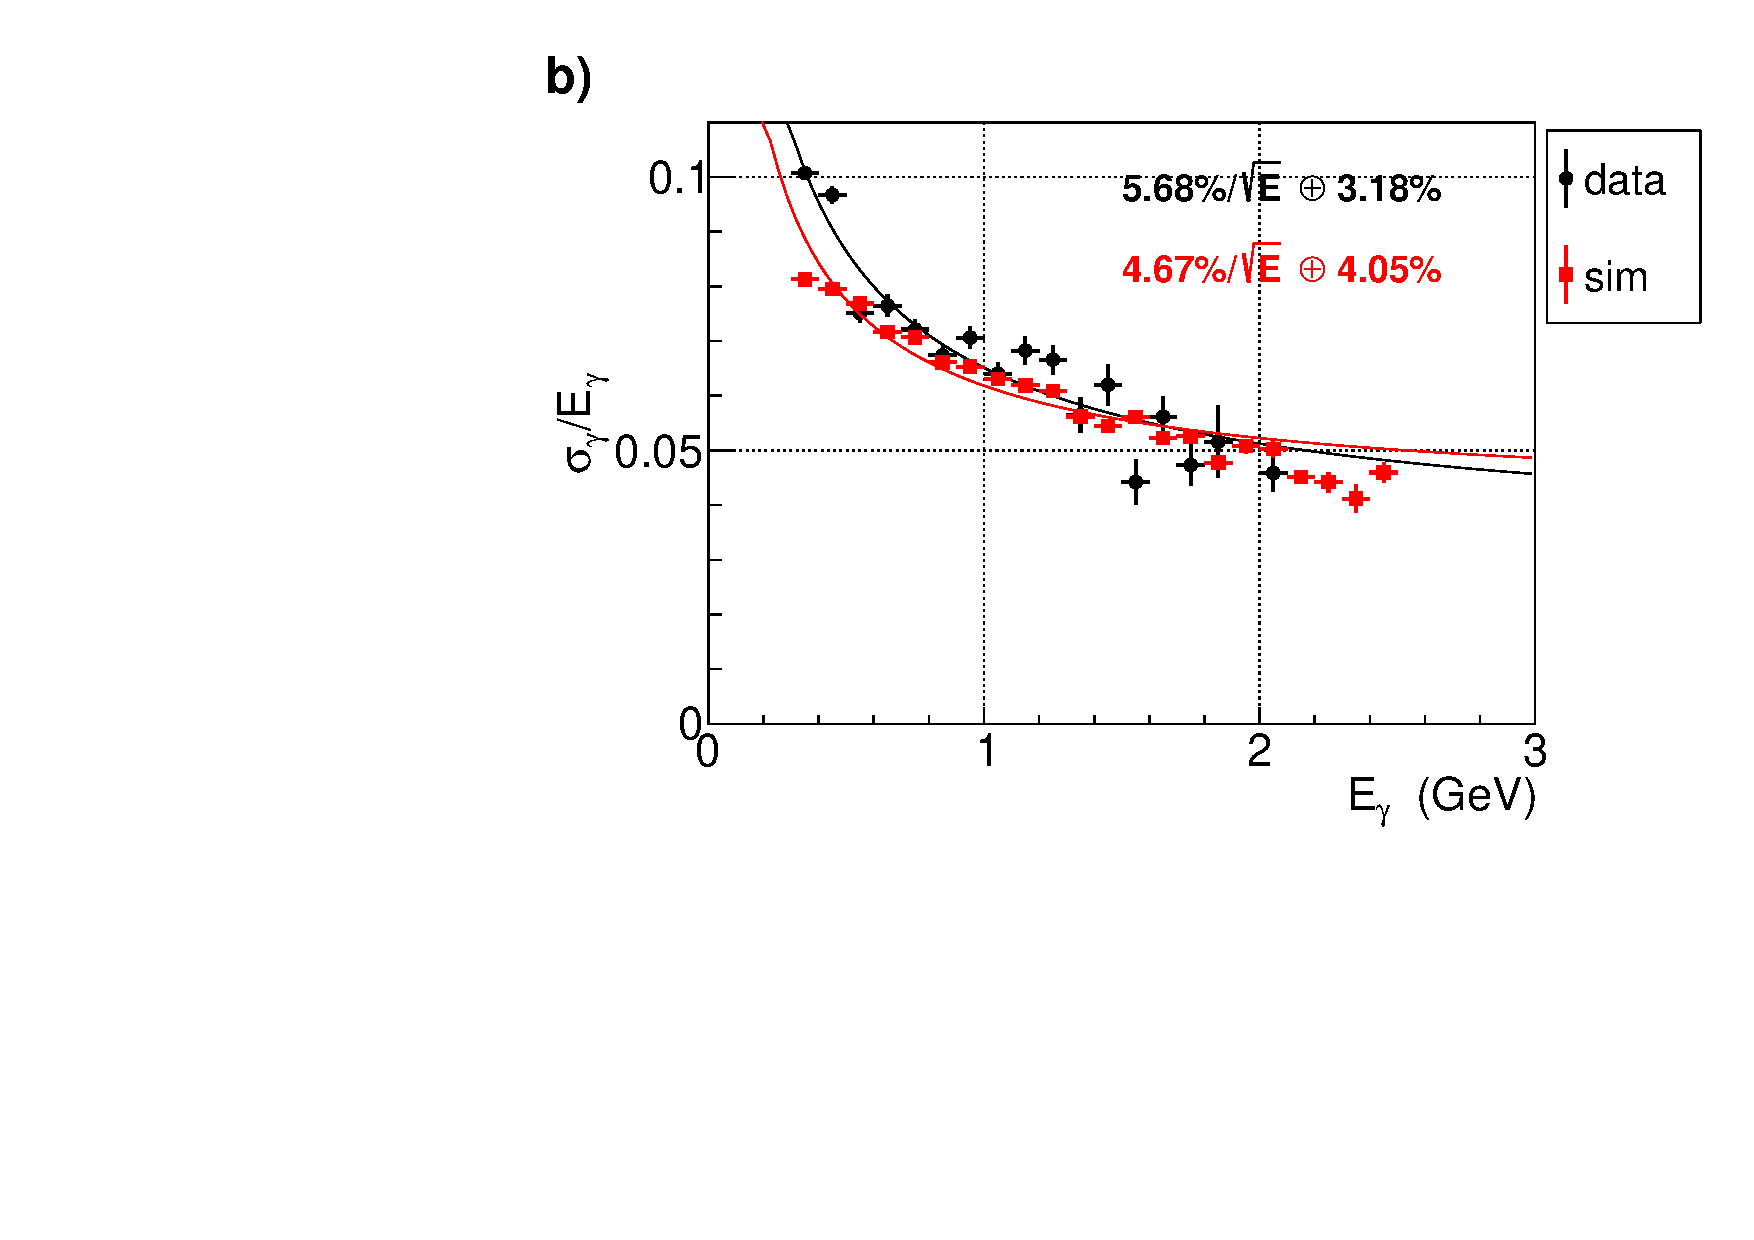
\includegraphics[width=0.45\textwidth]{figures/mcsmear50_37_gPsym100_E_sigma.pdf}
\caption{\label{fig:bcal:eta_resolution}
a)  Measured and simulated  $\eta$ width as a function of energy for symmetric decays, where both photons are required to be within 0.1 GeV of each other. 
b) The energy resolution of single photons calculated under the assumption that only the energy resolution contributes to the $\eta$ width. The curves are fits based on  Eq.\,\ref{eq:resolutionfit}.
(Color online)
 }
\end{figure}    






\subsection{Summary \label{sec:calsummary}}